\documentclass{article}

\usepackage{a4}
\usepackage{amsmath}
\usepackage{amssymb}
\usepackage{ctex}
\usepackage{booktabs}
\usepackage{graphicx}
\usepackage{float}
\usepackage{hyperref}
\usepackage{enumitem}
\usepackage{array}
\usepackage{fvextra}
\RecustomVerbatimEnvironment{verbatim}{Verbatim}{
  breaklines=true,
  breakanywhere=true,
  fontsize=\small
}

\hypersetup{colorlinks=true,linkcolor=black,urlcolor=blue,citecolor=black}
\setlist[itemize]{nosep,leftmargin=1.8em}
\setlist[enumerate]{nosep,leftmargin=1.8em}

\title{计算机体系结构\\实验4\\类 SRAM 与 AXI 总线}
\author{鲁昕宁 \quad 2414015}
\date{2026年11月18日}
\begin{document}

\maketitle
\begin{center}
\begin{tabular}{ll}
GitHub仓库 & \parbox[t]{0.72\textwidth}{\raggedright\url{SidneyLu/Computer-Architecture-NKU-CS/tree/master/lab4}} \\[0.6em]
班号 & \underline{0964} \\[0.6em]
授课教师 & \underline{董前琨} \\[0.6em]
\end{tabular}
\end{center}

\newpage

\section{实验目标}
本实验在实验 3 的五级流水线上，完成《CPU设计实战》第 8 章的三个实践任务。
流水线、CP0、异常与中断逻辑沿用实验 3，乘法器和除法器仍使用 Xilinx IP。
实验箱未连接，按说明跳过比特流生成与上板验证；功能正确性以 \texttt{func\_lab9} 的 trace 比对为准。

\begin{enumerate}
  \item 将 CPU 顶层改为类 SRAM 总线，在 \texttt{CPU\_CDE\_SRAM} 中通过随机延迟的 \texttt{func\_lab9}。
  \item 在 CPU 外侧完成类 SRAM 到 AXI 的封装，对外只保留一个 AXI 主端口，
        在 \texttt{CPU\_CDE\_AXI} 中先于固定设置下通过 \texttt{func\_lab9}。
  \item 修改 \texttt{RANDOM\_SEED}，在固定、短、长三种设置下测试随机延迟，并均能通过同一套功能测试。
\end{enumerate}

AXI 侧信号按实验平台连接，整条总线按 AXI3 实现。
取指通路和数据通路各自经 \texttt{sram2axi} 转换后，由 \texttt{axi\_crossbar\_2x1} 合并为一路主端口，
再经 SoC 的 \texttt{axi\_crossbar\_1x2} 按地址分到 confreg 与 RAM。

\section{实验原理}
类 SRAM 与 AXI 都把一次访问分成两步：先确认从设备收下地址，再拿到读数据或写完成响应。
中间可以插入任意多个时钟周期的等待；CPU 只等握手完成，不要求固定几个时钟周期返回。
取指口和数据口各自最多一条在途传输，须等上一次 \texttt{data\_ok} 或 AXI 响应结束，才能再发请求。

\subsection{类 SRAM 的两段握手}
取指口和数据口使用同一组信号。主设备给出请求和访问内容，从设备分两次握手回应。

\begin{center}
\small
\begin{tabular}{@{}llp{0.52\textwidth}@{}}
\toprule
信号 & 方向 & 含义 \\
\midrule
\texttt{req} & 主$\to$从 & 请求有效；须保持到出现 \texttt{addr\_ok}=1 的时钟周期 \\
\texttt{wr} & 主$\to$从 & 1 表示写 \\
\texttt{size} & 主$\to$从 & 0、1、2 分别对应字节、半字、字 \\
\texttt{wstrb} & 主$\to$从 & 写字节使能 \\
\texttt{addr}、\texttt{wdata} & 主$\to$从 & 地址和写数据 \\
\texttt{addr\_ok} & 从$\to$主 & 当前时钟周期已经收下这次请求 \\
\texttt{data\_ok} & 从$\to$主 & 这次请求完成；读访问时 \texttt{rdata} 有效 \\
\texttt{rdata} & 从$\to$主 & 读数据 \\
\bottomrule
\end{tabular}
\end{center}

\texttt{req}、\texttt{wr}、\texttt{size}、\texttt{wstrb}、地址和写数据在 \texttt{addr\_ok} 变为 1 之前保持不变。
\texttt{addr\_ok} 为 1 的时钟周期，从设备采样这些信号。下一时钟周期主设备拉低 \texttt{req}。
\texttt{sram\_wrap} 里，\texttt{ram\_en} 等于 \texttt{req} 与 \texttt{addr\_ok} 相与。
\texttt{req} 若在 \texttt{addr\_ok} 之后仍为 1，包装会再接受一次访问。

\texttt{data\_ok} 对应的是已经被接受的那一次，至少比这次 \texttt{addr\_ok} 延迟一个时钟周期。
读访问在 \texttt{data\_ok} 为 1 的时钟周期使用 \texttt{rdata}，CPU 把它锁存进 \texttt{fs\_inst} 或 \texttt{load\_buf}。
此后数据线上的变化属于下一次传输。

\subsection{从设备和地址}
指令口只连接 \texttt{sram\_wrap} 和指令 RAM，访问固定为字读：\texttt{wr} 为 0，\texttt{size} 为 2。
数据口先经过 \texttt{bridge\_1x2}，再分到数据 RAM 的 \texttt{sram\_wrap} 或 confreg。

RAM 包装的握手由掩码和一块返回缓冲决定：
\begin{verbatim}
assign addr_ok = addr_and && !buf_full_nxt;
assign data_ok = data_and && (!buf_empty || ram_en_r);
\end{verbatim}
\texttt{addr\_and} 和 \texttt{data\_and} 是分给该端口的两位随机掩码。
\texttt{ram\_en} 延迟一个时钟周期，记为 \texttt{ram\_en\_r}。
块 RAM 的读数据在这之后才随 \texttt{data\_ok} 送出。
同一次 RAM 请求的 \texttt{data\_ok} 因此比它的 \texttt{addr\_ok} 延迟至少一个时钟周期。

桥按下式判断 confreg 是否命中（掩码去掉地址 [31:29]，\texttt{0xbfafxxxx} 与 \texttt{0x1fafxxxx} 等价）：
\begin{verbatim}
wire hit_conf = (cpu_data_addr & 32'h1fff0000) == 32'h1faf0000;
\end{verbatim}
命中则访问 confreg，其余地址进数据 RAM。
\texttt{func\_lab9} 取指走 \texttt{0xbfc00000} 起的 kseg1，不经此桥。

桥在 \texttt{addr\_ok} 为 1 的时钟周期将选中的从设备记入 \texttt{sel\_conf\_reg}；
后续的 \texttt{data\_ok} 与 \texttt{rdata} 均从该侧返回。
该寄存器只记录最后一次被接受的访问目标。
若在上一次 \texttt{data\_ok} 之前再发新请求，响应可能与错误的一侧对应。
因此数据口上同时只能有一条在途访问。

confreg 自身不使用随机掩码。它的 \texttt{addr\_ok} 固定为 1，\texttt{data\_ok} 是请求延迟一个时钟周期后的 \texttt{conf\_req\_reg}。
写 LED、数码管这类地址时，请求发出的时钟周期就能被接受，完成响应在下一时钟周期。

\subsection{CPU 侧如何满足接口约束}
取指状态机为 \texttt{S\_IDLE}、\texttt{S\_REQ}、\texttt{S\_WAIT}、\texttt{S\_HAVE}、\texttt{S\_HOLD}。
只有 \texttt{S\_REQ} 把 \texttt{inst\_sram\_req} 置 1。\texttt{addr\_ok} 之后进入 \texttt{S\_WAIT}，\texttt{req} 在下一时钟周期为 0。
\texttt{data\_ok} 为 1 时锁存 \texttt{fs\_inst} 和 \texttt{fs\_pc}，再进入 \texttt{S\_HAVE}。译码级读的是这组锁存。
复位后的第一条请求地址是 \texttt{0xbfc00000}。离开 \texttt{S\_HAVE} 时，下一条地址在分支成立时取 \texttt{br\_target}，否则取当前 PC 加 4。

执行级访存状态机为 \texttt{D\_IDLE}、\texttt{D\_REQ}、\texttt{D\_WAIT}、\texttt{D\_DONE}、\texttt{D\_DROP}。
只有本级有效、本级无异常、且访存类型不是空操作时才进入 \texttt{D\_REQ}：
\begin{verbatim}
wire es_mem_go = es_valid && !es_ex_f && (es_mem_op != `MEM_NONE);
\end{verbatim}
字节、半字、字的 \texttt{size} 仍是 0、1、2，写选通沿用实验 3 的 \texttt{st\_wen}。
\texttt{wr} 在 \texttt{st\_wen} 非 0 时为 1。未到 \texttt{D\_DONE} 时 \texttt{es\_ready\_go} 为 0，指令留在执行级。
\texttt{data\_ok} 把读数据写入 \texttt{load\_buf}，访存级之后使用这份锁存。
在执行级就已经确定异常的指令不会进入 \texttt{D\_REQ}，因此 \texttt{SYSCALL} 后面被取消的 \texttt{sw} 不会出现在数据口上。

清空流水线时，按请求是否已被接受分开处理。
尚在请求态且本时钟周期没有 \texttt{addr\_ok} 时，取指改地址，访存回到 \texttt{D\_IDLE}。
已经接受而 \texttt{data\_ok} 尚未返回时，取指置 \texttt{kill}，访存进入 \texttt{D\_DROP}。
两者都把这次返回丢掉，从设备侧仍然是一次接受对应一次 \texttt{data\_ok}。
写回级还没给出入口、执行级已经取消后续指令时，取指停在 \texttt{S\_HOLD}，有了入口地址再发请求。

下一条取指地址在离开 \texttt{S\_HAVE} 时才确定，所以分支目标必须等延迟槽已经取回。
译码级看到分支或跳转时，等到取指级送来的 PC 等于本指令 PC 加 4：
\begin{verbatim}
wire bd_arrived = fs_to_ds_valid && (fs_pc == ds_pc + 32'd4);
wire wait_bd    = ds_is_bj && !bd_arrived;
assign ds_ready_go = ~load_use && ~mfc_use && ~wait_bd;
\end{verbatim}
\texttt{br\_taken} 以 \texttt{ds\_ready\_go} 为前提，目标只在该时钟周期被取指级采样。
送入下一条的 BD 位来自当前译码级中的转移指令。带 BD 的异常处理沿用实验 3，EPC 为异常指令 PC 减 4。

\subsection{随机延迟只作用在握手上}
任务三通过改写宏 \texttt{RANDOM\_SEED} 检查随机延迟。后文统一称写入 \texttt{confreg} 的 23 位初值为种子（高 7 位取 \texttt{7'b1010101}，低 16 位在仿真前改写），称固定、短、长三种掩码工作方式为设置（由复位结束时锁存的 \texttt{no\_mask}、\texttt{short\_delay} 决定），称类 SRAM 顶层、AXI 转接桥封装、原生 AXI 为三个实验组。

\texttt{confreg} 在复位期间装入种子，驱动 23 位线性反馈移位寄存器逐时钟周期推进。
复位保持一个时钟周期以上后，从种子低位得到两个标志：低 16 位为 \texttt{16'h00FF} 时 \texttt{no\_mask} 为 1；低 8 位为 \texttt{8'hFF} 时 \texttt{short\_delay} 为 1。
据此，种子低 16 位 \texttt{16'h00FF} 对应固定设置，\texttt{no\_mask} 把五位掩码或成 1；\texttt{16'h01FF} 对应短设置，\texttt{short\_delay} 为 1 而 \texttt{no\_mask} 为 0；\texttt{16'h0000} 对应长设置，两个标志都为 0。

五位掩码 \texttt{ram\_random\_mask} 由移位寄存器当前状态和上述两个标志共同给出。
固定设置下掩码恒为 1，握手只受接口协议本身约束。
短设置和长设置下掩码会随移位寄存器变化；长设置对掩码位的约束更紧，掩码为 0 的时钟周期更多，握手需要多等。

类 SRAM 的指令包装使用掩码低两位，数据 RAM 包装使用其上的两位；
在同一侧内，较高位控制 \texttt{addr\_ok}，较低位控制 \texttt{data\_ok}。
环境默认种子的低 16 位是 \texttt{16'h01FF}，对应短设置。
confreg 不经过这组掩码。

AXI 的 \texttt{axi\_wrap\_ram} 使用全部 5 位：bit 4 到 bit 0 依次作用在 AR、R、AW、W、B 上。
AR、AW、W 在 \texttt{valid} 置 1 之后把对应的 \texttt{*\_nomask} 置 1，并保持到该通道握手。
这段时间里 \texttt{valid} 由该保持位维持为 1。
R、B 每个时钟周期与掩码相与，\texttt{rvalid}、\texttt{bvalid} 可以在相邻两个时钟周期之间变为 0。
功能测试未定义 \texttt{RUN\_PERF\_TEST}，故 \texttt{axi\_wrap\_ram} 启用上述随机掩码。
工程里保存的种子是 \texttt{\{7'b1010101,16'h00FF\}}，对应固定设置。
三种设置下的仿真安排和通过情况见实验结果。

\subsection{AXI 协议在本实验中的体现}
AXI 把一次访问拆到若干条通道上。读事务走读地址通道 AR 和读数据通道 R，写事务走写地址通道 AW、写数据通道 W 和写响应通道 B。每条通道单独握手：源端保持 \texttt{valid} 以及该通道上的地址或数据，直到 \texttt{ready} 为 1；两者同时为 1 的时钟周期，这一次传递完成。

读和写占用不同的通道，所以一笔读事务和一笔写事务可以同时进行。每笔事务带有 ID，从设备在 R 或 B 上送回同一个 ID，主设备据此把响应交还给发出它的那一路。\texttt{rlast} 和 \texttt{wlast} 标出这笔事务的数据已经传完。

本实验对外是 AXI3，地址和数据都是 32 位。类 SRAM 的一次访问对应总线上的一次数据传递：读的时候 \texttt{rlast} 为 1，写的时候 \texttt{wlast} 为 1。\texttt{arlock}、\texttt{awlock}、\texttt{cache}、\texttt{prot} 和 QoS 接 0。功能测试里从设备返回 OKAY，状态机按 \texttt{valid} 与 \texttt{ready} 推进。写数据通道上的 \texttt{wid} 留在顶层端口。

\subsection{类 SRAM 接口与 AXI 的关系}
类 SRAM 是 CPU 核上的接口，信号为一组 \texttt{req}、\texttt{wr}、\texttt{size}、\texttt{addr}、\texttt{wdata} 和 \texttt{addr\_ok}、\texttt{data\_ok}、\texttt{rdata}。地址在 \texttt{addr\_ok} 为 1 时被收下，读数据或写完成在 \texttt{data\_ok} 为 1 时交还。同一端口上读和写共用这组信号，同时只保留一条在途访问。它没有 AR、R、AW、W、B 五条通道，也没有事务 ID。因此类 SRAM 不是 AXI 的一种简化命名，实验里也不另设称为类 AXI 的总线。

一次类 SRAM 访问和一笔 AXI 事务的对应，由转接桥来做。流水级继续用任务一的状态机，\texttt{sram2axi} 把一次 \texttt{req} 到 \texttt{data\_ok} 收成一笔 AXI3 事务：读走 AR 和 R，写走 AW、W 和 B。\texttt{addr\_ok} 在转换器收下请求的那个时钟周期为 1，\texttt{arvalid} 或 \texttt{awvalid} 再延迟一个时钟周期。\texttt{mycpu\_top} 引出的已经是 AXI 主端口，SoC 上的 Crossbar、\texttt{axi\_ram} 和 confreg 按 AXI 接收。

原生实现去掉这层转接。取指级直接驱动 AR 和 R，执行级直接驱动 AR/R 或 AW/W/B，核内不再出现 \texttt{req} 与 \texttt{data\_ok}。对外仍是同一个 AXI3 主端口，ID 的用法与转接桥相同。两种实现的差别在于五条通道由转换器驱动还是由流水级驱动。

\subsection{AXI 的五个通道}
下表列出五条通道在本设计中的方向和用法。通道在 \texttt{valid} 与 \texttt{ready} 同时为 1 时完成传递，在此之前源端保持 \texttt{valid} 以及地址或数据。

\begin{center}
\small
\begin{tabular}{@{}llp{0.48\textwidth}@{}}
\toprule
通道 & 方向 & 本设计的用法 \\
\midrule
AR & 主$\to$从 & 读地址，\texttt{arburst}=\texttt{2'b01} \\
R & 从$\to$主 & 一次读数据，\texttt{rlast}=1 \\
AW & 主$\to$从 & 写地址，与 W 同时发出 \\
W & 主$\to$从 & 写数据和 \texttt{wstrb}，\texttt{wlast}=1 \\
B & 从$\to$主 & 写响应。握手所在时钟周期产生 \texttt{data\_ok} \\
\bottomrule
\end{tabular}
\end{center}

AR 的 \texttt{arburst} 接 \texttt{2'b01}，即 INCR。
\texttt{arsize}、\texttt{awsize} 由类 SRAM 的 \texttt{size} 在高位补 0 得到，\texttt{wstrb} 原样送出。
从设备握手时返回 OKAY。转换器根据 \texttt{valid}、\texttt{ready} 和 \texttt{rlast} 决定进入下一状态的时刻。

\subsection{一次类 SRAM 访问对应一次 AXI 事务}
流水级仍然只看见类 SRAM。\texttt{sram2axi} 放在 \texttt{mycpu\_core} 外面，把 \texttt{addr\_ok} 与 \texttt{data\_ok} 这两段握手接到五条通道上。取指和数据各有一份转换器，每份同时只做一笔事务，两份的状态互不影响。

转换器空闲且 \texttt{req} 为 1 时，同一时钟周期给出 \texttt{addr\_ok}，并把 \texttt{size}、\texttt{wstrb}、\texttt{addr}、\texttt{wdata} 锁存下来。
下一时钟周期 CPU 拉低 \texttt{req}，转换器离开空闲，\texttt{addr\_ok} 回到 0。
此后 AR、AW、W 都用锁存值，CPU 再改地址也不会改到已经发出的事务。

读请求进入 \texttt{A\_AR}，拉高 \texttt{arvalid}。\texttt{arready} 到来后进入 \texttt{A\_R}，拉高 \texttt{rready}。
\texttt{rvalid}、\texttt{rready}、\texttt{rlast} 同时为 1 的时钟周期，\texttt{data\_ok} 为 1，\texttt{rdata} 在这一时钟周期被取走，然后回到空闲。

写请求进入 \texttt{A\_WRITE}，\texttt{awvalid} 和 \texttt{wvalid} 一起拉高。
\texttt{aw\_done} 和 \texttt{w\_done} 分别记下两个通道是否已经握手，先完成的那一路把 \texttt{valid} 拉低，握手只发生一次。
两路都完成后进入 \texttt{A\_WRESP}。\texttt{bvalid} 与 \texttt{bready} 同时为 1 时 \texttt{data\_ok} 为 1，随即回到空闲。
\texttt{arid}、\texttt{awid}、\texttt{wid} 以及 \texttt{arlock}、\texttt{awlock}、\texttt{cache}、\texttt{prot} 都接 0。

\subsection{原生 AXI 接口}
原生 AXI 指流水级直接驱动五条通道，完成条件就是通道握手，核内不另设类 SRAM 的 \texttt{req} 与 \texttt{data\_ok}。
取指级需要下一条指令时拉高 \texttt{arvalid}，
地址和 \texttt{arid} 保持到 \texttt{arready}。
随后拉高 \texttt{rready}，在 \texttt{rvalid} 与 \texttt{rlast} 同时为 1 的时钟周期把 \texttt{rdata} 锁进 \texttt{fs\_inst}。
访存级对 load 走同一套 AR/R；对 store 同时拉高 \texttt{awvalid} 与 \texttt{wvalid}，两通道各自握手后再等 \texttt{bvalid}。
执行级在 R 或 B 完成之前 \texttt{es\_ready\_go} 为 0，与现在停在 \texttt{D\_WAIT} 的作用相同。

对外仍只能有一个 AXI 主端口，取指和访存仍会同时发出事务，所以原生接口并不能省掉合并。
两条通路要在核内共用一组 AR/R/AW/W/B，或者各自形成一路 AXI 再接入 Crossbar。
前一种做法把仲裁写进流水级：两路同时要读地址时只允许一路 \texttt{arvalid} 为 1，另一路停在发地址状态；
\texttt{arid}/\texttt{awid} 仍须区分来源，R/B 按 ID 送回对应的流水级。
后一种做法的主端口行为与现在的 \texttt{axi\_crossbar\_2x1} 相同，差别只在状态机位于 \texttt{IF\_stage}、\texttt{EXE\_stage} 内部，而不是位于 \texttt{sram2axi}。

清空流水线和延迟槽的约束也不因接口而改变。
\texttt{arvalid}、\texttt{awvalid}、\texttt{wvalid} 拉高之后一直保持到对应的 \texttt{ready}，地址和写数据在这期间不变。
清空时把该时钟周期标为丢弃：读数据返回后不写入指令寄存器，写响应返回后执行级回到空闲。
新的取指地址记在挂起的 PC 里，等当前读事务结束再发。
分支目标仍须等延迟槽的取指事务完成后再发，否则目标会早于槽内指令出现在 AR 通道上。

\begin{center}
\small
\begin{tabular}{@{}p{0.22\textwidth}p{0.36\textwidth}p{0.32\textwidth}@{}}
\toprule
 & 现用的类 SRAM 封装 & 原生 AXI \\
\midrule
流水级看到的完成条件 & \texttt{addr\_ok} 之后的 \texttt{data\_ok} & R 的 \texttt{rlast} 或 B 握手 \\
AXI 通道的宿主 & 核外两份 \texttt{sram2axi} & \texttt{IF\_stage} 与 \texttt{EXE\_stage} \\
两路合并 & \texttt{axi\_crossbar\_2x1} & 核内仲裁，或同样使用 Crossbar \\
与任务一的关系 & 直接复用 \texttt{mycpu\_core} & 须重写取指和访存状态机 \\
\bottomrule
\end{tabular}
\end{center}

默认综合采用前一列。任务一已在类 SRAM 上通过随机延迟，任务二的单主端口由封装接出。

原生路径另写 \texttt{if\_stage\_axi} 与 \texttt{exe\_stage\_axi}，组成 \texttt{mycpu\_core\_axi}，仍接原译码、访存、写回。
宏 \texttt{NATIVE\_AXI} 打开后，流水级直接驱动通道。
两路仍进同一颗 \texttt{axi\_crossbar\_2x1}，线程 ID 为 0，基址 ID 仍为 0 和 8。
两种做法的写回都由指令语义决定。
封装在 \texttt{addr\_ok} 与通道 \texttt{valid} 之间多延迟一个时钟周期；从设备侧的等待两种路径都要承受。
固定设置下的时间与通道对照见实验结果。
\texttt{NATIVE\_AXI} 不写入工程默认宏，日常仿真仍走转接桥加 Crossbar。

\subsection{为何采用 Crossbar}
任务二要求 CPU 对外只呈现一个 AXI 主端口，而 \texttt{mycpu\_core} 在任务一中已是取指、访存两条独立的类 SRAM 主口。
每条口各维护一条在途传输，\texttt{addr\_ok} 与 \texttt{data\_ok} 也分别在 \texttt{IF\_stage} 与 \texttt{EXE\_stage} 中处理。
若把两路 AXI 信号直接拼在一根总线上，或用简单多路选择器轮流服务，会出现三类问题：
读地址通道无法在无 ID 的情况下区分响应应回到哪一路 \texttt{sram2axi}；
两路同时需要读地址时缺乏规范的仲裁与反压，取指与访存会互相阻塞对方的 \texttt{arready}；
写通道与读通道在 AXI 上本就分离，简单合并难以在保持单次传输的事务语义的同时允许取指读与数据写并行推进。

因此用两颗 Crossbar 分工：核外 \texttt{2$\times$1} 合并取指与数据，SoC 内 \texttt{1$\times$2} 按地址选从设备。
核外的 \texttt{axi\_crossbar\_2x1} 把两份 \texttt{sram2axi} 合成一路主端口：
S00 接取指、S01 接数据，并为两路配置不同的仲裁优先级与基址 ID，使 R/B 能按 ID 回到发起事务的那一侧。
SoC 上原有的 \texttt{axi\_crossbar\_1x2} 则按地址窗口把该主端口的事务送到 confreg 或 \texttt{axi\_ram}，
与实验平台提供的顶层结构一致，避免在自写转接桥里重复实现设备译码。
早期亦可用转接桥内部轮询合并两路；功能上能通过 \texttt{func\_lab9}，但仲裁与流水细节都挤在桥内，且与平台 Crossbar 的仿真路径不一致。
改为 IP Crossbar 后，固定设置下到达第 94 点的时间约增加 4.8\,ms，写回 trace 仍为 94/94，
说明多出的时钟周期来自 Crossbar 的寄存与仲裁，而非功能错误。

\subsection{两路并成一个主端口}
CPU 核心仍是类 SRAM 接口。AXI 顶层在核心外放两份 \texttt{sram2axi}，经 \texttt{axi\_crossbar\_2x1} 合成一个主端口；
该主端口再接入 SoC 的 \texttt{axi\_crossbar\_1x2}，由后者按地址分发到 confreg 与 RAM。

\texttt{axi\_crossbar\_2x1} 是 2 个从接口、1 个主接口，协议 AXI3，地址和数据都是 32 位。
主接口 ID 为 4 位。每个从接口在总线上占 4 位，其中低 3 位是线程号，转换器把线程号接 0。
Crossbar 给 S00 的基址 ID 为 0，给 S01 的基址 ID 为 8。
因此主端口上取指事务的 ID 为 0，数据事务的 ID 为 8。R、B 按这个 ID 送回原来的从端口。
2$\times$1 的主端口地址从 0 起，覆盖全部 32 位，本身不做设备译码。

取指接 S00，仲裁优先级为 0。数据接 S01，仲裁优先级为 15。
两路同时把 \texttt{arvalid} 拉高时，Crossbar 先接受数据口。取指停在 \texttt{A\_AR}，\texttt{arvalid} 保持到自己的 \texttt{arready}。
读通道和写通道相互独立，所以主端口上可以同时有一条取指读和一条数据写。下游 RAM 的读、写也各自独立。

1$\times$2 负责设备译码。confreg 有两段 16 位窗口，基址为 \texttt{0x1faf0000} 和 \texttt{0xbfaf0000}。
RAM 的窗口为 22 位，其中包括 \texttt{0x1fc00000} 和程序实际取指用的 \texttt{0xbfc00000}。
顶层保留 \texttt{wid}，即 AXI3 写数据通道上的 ID。

\subsection{和 AXI4 的差别}
CPU 经 \texttt{sram2axi} 发起的事务在 AXI4 下同样合法，lock 接 0，\texttt{wlast} 为 1。
SoC 端口宽度按 AXI3 例化，两颗 Crossbar 的协议选项亦为 AXI3。

\begin{center}
\small
\begin{tabular}{@{}p{0.24\textwidth}p{0.34\textwidth}p{0.32\textwidth}@{}}
\toprule
信号 & 本设计（AXI3） & AXI4 标准 \\
\midrule
\texttt{wid} & 有，4 位 & 写数据不再带独立 ID \\
\texttt{arlock}、\texttt{awlock} & 2 位，驱动为 0 & 1 位 \\
\texttt{arqos}、\texttt{awqos} & 从端口接 0，主端口不引出 & 接口上有这 4 位 \\
\bottomrule
\end{tabular}
\end{center}

\section{实验过程}
环境来自 \texttt{lab10.zip}（类 SRAM）与 \texttt{lab11.zip}（AXI）。
将实验 3 的 \texttt{func\_lab9} 复制到两边的 \texttt{soft/func\_lab9}，令 \texttt{inst\_ram}、\texttt{axi\_ram} 的 coe 指向同一 \texttt{inst\_ram.coe}。
目标器件 \texttt{xc7a200tfbg676-2}，工具 Vivado 2025.1；在压缩包自带的 \texttt{mycpu.xpr} 上展开工程，\texttt{axi\_crossbar\_2x1} 放在 AXI 工程 \texttt{rtl/xilinx\_ip} 下。

\texttt{golden\_trace.txt} 由 \texttt{cpu132\_gettrace} 在固定设置下生成，与随机种子无关。
类 SRAM 环境生成一次，AXI 环境共用，仿真顶层均为 \texttt{tb\_top}。
CPU 核心 RTL 在 \texttt{CPU\_CDE\_SRAM/.../rtl/myCPU}；AXI 工程复用 \texttt{mycpu\_core}，在 \texttt{mycpu\_top} 外挂双路 \texttt{sram2axi} 与 Crossbar。

仿真顺序如下。
类 SRAM 实验组在固定、短、长三种设置下各跑全量 \texttt{func\_lab9}，种子恢复为 \texttt{16'h01FF}。
AXI 转接桥实验组三种设置依次验证后，在固定设置下用 Crossbar 复测。
再打开 \texttt{NATIVE\_AXI}，三种设置各测一遍，种子恢复为 \texttt{16'h00FF}。
波形图取自 4500 个时钟周期的短仿真（类 SRAM 用短设置、AXI 用固定设置），宏 \texttt{WAVE\_DUMP} 仅用于出图，94 点回归不打开。
时钟编号从 \texttt{resetn} 释放后的首个 CPU 沿算起（周期 10\,ns，第 1 个沿约 2005\,ns）。

\section{关键代码}
本节摘录与原理对应的状态机与连线。类 SRAM 握手在 \texttt{IF\_stage}、\texttt{EXE\_stage}；AXI 转换在 \texttt{sram2axi}，合并在 \texttt{mycpu\_top}。
类 SRAM 顶层将 \texttt{hw\_int} 接 0；AXI 顶层接 SoC 中断，核外例化两份 \texttt{sram2axi} 与 Crossbar。取指与访存各有一条在途传输。

\subsection{取指状态机}
请求只在 \texttt{S\_REQ} 为高，地址用 \texttt{req\_pc}，写使能为 0，宽度固定为一个字。
译码级看到的是锁存后的 \texttt{fs\_inst} 和 \texttt{fs\_pc}。
\texttt{fs\_valid} 为 1 且译码级允许进入、当前时钟周期也没有清空流水线时，\texttt{fs\_fire} 为 1，本条指令离开取指级。

\begin{center}
\small
\begin{tabular}{@{}llp{0.48\textwidth}@{}}
\toprule
状态 & 请求 & 转移 \\
\midrule
\texttt{S\_IDLE} & 无 & 下一时钟周期进入 \texttt{S\_REQ}，地址为 \texttt{0xbfc00000} \\
\texttt{S\_REQ} & 有 & \texttt{addr\_ok} 后进入 \texttt{S\_WAIT}，并保存 \texttt{acc\_pc} \\
\texttt{S\_WAIT} & 无 & \texttt{data\_ok} 后锁存，进入 \texttt{S\_HAVE} \\
\texttt{S\_HAVE} & 无 & \texttt{fs\_fire} 后回到 \texttt{S\_REQ}，发出下一条 \\
\texttt{S\_HOLD} & 无 & 入口地址到达后回到 \texttt{S\_REQ} \\
\bottomrule
\end{tabular}
\end{center}

复位时 \texttt{fs\_pc} 置为 \texttt{0xbfbffffc}，\texttt{fs\_valid} 为 0，第一条请求地址单独写成 \texttt{0xbfc00000}。
\texttt{S\_HAVE} 里下一条地址是：
\begin{verbatim}
req_pc <= br_taken ? br_target : (fs_pc + 32'd4);
\end{verbatim}
\texttt{br\_taken} 已经等延迟槽到齐，所以这里采样到的目标就是本条转移指令的目标。

清空流水线的时钟周期先把入口写入 \texttt{pend\_pc}，并把 \texttt{fs\_valid} 清 0，译码级不再收下当前指令。
请求还在 \texttt{S\_REQ}、该时钟周期又没有 \texttt{addr\_ok} 时，\texttt{req\_pc} 同时改成 \texttt{wb\_flush\_pc}。
\texttt{pend\_flush} 留到下一时钟周期：若仍未接受，就再用 \texttt{pend\_pc} 作为地址并清掉该标志；
若该时钟周期已经被接受，则 \texttt{kill} 为 1，返回的指令丢弃，\texttt{data\_ok} 之后按 \texttt{pend\_pc} 再发一次。
已经进入 \texttt{S\_WAIT} 时地址不能再改，只把 \texttt{kill} 置 1，\texttt{data\_ok} 后丢弃 \texttt{inst\_sram\_rdata}。
写回级若在该时钟周期给出入口，就立刻重新请求；入口还在 \texttt{pend\_pc} 里，就用它再发一次。
只有执行级已经取消、入口尚未产生时才进入 \texttt{S\_HOLD}。
\texttt{S\_HOLD} 不发请求，\texttt{wb\_flush} 或 \texttt{pend\_flush} 提供地址后再回到 \texttt{S\_REQ}。

\texttt{addr\_ok} 与清空发生在同一个时钟周期，请求已经被从设备接受，进入 \texttt{S\_WAIT} 时 \texttt{kill} 为 1。
每次被接受的取指都会等到自己的 \texttt{data\_ok}，下一次请求才发出。

\subsection{访存状态机}
访存请求的地址是 \texttt{alu\_result}，写数据是按字节或半字展开后的 \texttt{st\_data}。
\texttt{st\_wen} 非 0 时 \texttt{wr} 为 1，写选通直接用 \texttt{st\_wen}。
\texttt{LB}、\texttt{LBU}、\texttt{SB} 的 \texttt{size} 为 0，\texttt{LH}、\texttt{LHU}、\texttt{SH} 为 1，其余访存为 2。
\begin{verbatim}
wire mem_wait = es_mem_go && (dst != D_DONE);
assign es_ready_go = mem_wait ? 1'b0 :
    ((es_is_mul | es_is_divop) ? md_ready : 1'b1);
assign data_sram_req = (dst == D_REQ);
\end{verbatim}
访存未完成时 \texttt{es\_ready\_go} 为 0，执行级留在当前指令上。
没有访存时，乘除法仍等 \texttt{md\_ready} 再离开执行级。

\texttt{D\_IDLE} 在需要访存时进入 \texttt{D\_REQ}。
\texttt{addr\_ok} 之后进入 \texttt{D\_WAIT}。
\texttt{data\_ok} 时把读数据写入 \texttt{load\_buf}，再进入 \texttt{D\_DONE}。
访存级允许接收后回到 \texttt{D\_IDLE}。store 也经过这些状态。
\texttt{load\_buf} 对 store 没有用途，写回级不采用这份数据。

清空流水线的优先级写在正常转移之前，按请求是否已经被接受分开：
\begin{verbatim}
wb_flush && D_REQ && !addr_ok -> D_IDLE
wb_flush && (D_REQ && addr_ok || D_WAIT) -> D_DROP
wb_flush && (D_DONE || D_IDLE) -> D_IDLE
\end{verbatim}
\texttt{D\_DROP} 只等 \texttt{data\_ok}，不写入 \texttt{load\_buf}，然后回到 \texttt{D\_IDLE}。
\texttt{es\_mem\_go} 要求 \texttt{es\_ex\_f} 为 0，所以在执行级就已经确定异常的指令不会进入 \texttt{D\_REQ}。
\texttt{SYSCALL} 之后的 \texttt{sw} 属于被取消的后续指令，数据口上看不到这次写。

\subsection{sram2axi}
\texttt{sram2axi} 把一次类 SRAM 访问转换成一次 AXI3 传输。取指和数据各例化一次，状态互不影响。
离开空闲之前，先把 \texttt{size}、\texttt{wstrb}、\texttt{addr}、\texttt{wdata} 锁存到寄存器，后面的 AXI 地址和数据都用这些值。

\begin{center}
\small
\begin{tabular}{@{}llp{0.46\textwidth}@{}}
\toprule
状态 & AXI 信号 & 转移 \\
\midrule
\texttt{A\_IDLE} & 无 valid & \texttt{req} 为 1 时，写去 \texttt{A\_WRITE}，读去 \texttt{A\_AR} \\
\texttt{A\_AR} & \texttt{arvalid} & \texttt{arready} 后进入 \texttt{A\_R} \\
\texttt{A\_R} & \texttt{rready} & \texttt{rvalid} 且 \texttt{rlast} 后回到空闲 \\
\texttt{A\_WRITE} & \texttt{awvalid}、\texttt{wvalid} & AW 与 W 都握手后进入 \texttt{A\_WRESP} \\
\texttt{A\_WRESP} & \texttt{bready} & \texttt{bvalid} 后回到空闲 \\
\bottomrule
\end{tabular}
\end{center}

空闲且 \texttt{req} 为 1 时，\texttt{addr\_ok} 在该时钟周期为 1。
CPU 的取指或访存状态机同时离开请求态，下一时钟周期 \texttt{req} 为 0，转换器也离开空闲，\texttt{addr\_ok} 随之变 0。
\begin{verbatim}
assign addr_ok = (st == A_IDLE) && req;
assign data_ok = read_fire || b_fire;
assign arsize  = {1'b0, size_r};
assign arburst = 2'b01;
\end{verbatim}
\texttt{read\_fire} 是 \texttt{A\_R} 中 \texttt{rvalid \&\& rready \&\& rlast}，\texttt{b\_fire} 是 \texttt{A\_WRESP} 中 \texttt{bvalid \&\& bready}。
读回的数据就是该时钟周期的 \texttt{rdata}。
CPU 把它锁存进 \texttt{fs\_inst} 或 \texttt{load\_buf}。

写通道用 \texttt{aw\_done} 和 \texttt{w\_done} 分别记住 AW、W 是否已经握手。
某个时钟周期两者同时被接受时，条件里把“本时钟周期的握手”和“先前已经完成”合在一起判断，因此不必再等一个时钟沿才进入 \texttt{A\_WRESP}。
\texttt{awvalid} 在 \texttt{aw\_done} 之后拉低，\texttt{wvalid} 在 \texttt{w\_done} 之后拉低，避免已经接受的通道再被握手一次。
\texttt{wlast} 固定为 1。\texttt{arid}、\texttt{awid}、\texttt{wid} 固定为 0。
\texttt{arlock}、\texttt{awlock}、\texttt{arcache}、\texttt{awcache}、\texttt{arprot}、\texttt{awprot} 固定为 0。
返回的 \texttt{rid}、\texttt{rresp}、\texttt{bid}、\texttt{bresp} 不参与状态转移。

\subsection{Crossbar 的连接}
两份 \texttt{sram2axi} 的 AXI 信号按 \{数据, 取指\} 拼成 Crossbar 的从端口，低位是 S00。
每个从端口在总线上占 \texttt{ID\_WIDTH} 即 4 位，其中低 3 位接转换器的线程号，最高位接 0：
\begin{verbatim}
.s_axi_araddr ({d_araddr, i_araddr}),
.s_axi_arvalid({d_arvalid, i_arvalid}),
.s_axi_arid   ({1'b0, d_arid, 1'b0, i_arid}),
\end{verbatim}
Crossbar 返回的 \texttt{rid}、\texttt{bid} 也是每路 4 位。
转换器只接收低 3 位，而且状态机不看它们。
\texttt{arqos} 和 \texttt{awqos} 在从端口接 0。
主端口的 QoS 不连接，因此不会送到 SoC。

S01 的仲裁优先级是 15，S00 是 0。
数据口和取指口同时把 \texttt{arvalid} 拉高时，Crossbar 先接受数据口；取指口保持 \texttt{arvalid}，停在 \texttt{A\_AR}，直到自己的 \texttt{arready} 到来。
两个转换器各有一次未完成的传输，所以主端口上可以同时有一路读和一路写。
Crossbar 给取指响应的 ID 带基址 0，给数据响应的 ID 带基址 8，再按这个 ID 把 R 或 B 送回原来的从端口。

\section{实验结果}
仿真在每条写回有效且目标寄存器非 0 时，把 PC、寄存器号和写数据与 \texttt{golden\_trace.txt} 比较；94 个功能点一致则打印 \texttt{----PASS!!!}。
\texttt{gettrace} 在第 94 点止于 2130615\,ns，与实验 3 参考轨迹一致。
下表汇总各方案的首次与末次测试点时间（墙钟时间，单位 ns）。

\begin{center}
\small
\begin{tabular}{lrrl}
\toprule
方案 & 第 1 点 & 第 94 点 & 结果 \\
\midrule
gettrace & 14055\,ns & 2130615\,ns & 生成轨迹 \\
类 SRAM，固定设置 & 38055\,ns & 5358945\,ns & 94/94 \\
类 SRAM，短设置 & 96805\,ns & 13963675\,ns & 94/94 \\
类 SRAM，长设置 & 183735\,ns & 26413855\,ns & 94/94 \\
AXI 转接桥，固定设置 & 74285\,ns & 10881865\,ns & 94/94 \\
AXI 转接桥，短设置 & 119455\,ns & 17765195\,ns & 94/94 \\
AXI 转接桥，长设置 & 187165\,ns & 27821755\,ns & 94/94 \\
AXI Crossbar，固定设置 & 110065\,ns & 15681855\,ns & 94/94 \\
原生 AXI，固定设置 & 98075\,ns & 13969665\,ns & 94/94 \\
\bottomrule
\end{tabular}
\end{center}

固定设置下，Crossbar 封装比单纯转接桥晚约 4.80\,ms 到第 94 点，差额在 Crossbar 的仲裁与寄存。
原生 AXI 在同一设置下第 1 点 98075\,ns、第 94 点 13969665\,ns，亦为 94/94；相对 Crossbar 封装，第 94 点提前约 1.71\,ms，主要来自去掉 \texttt{sram2axi} 在 \texttt{addr\_ok} 与通道 \texttt{valid} 之间多出的一个时钟周期，Crossbar 与 RAM 侧的等待仍在。

\subsection{随机延迟验证}
类 SRAM、AXI 转接桥与原生 AXI 三个实验组各在固定、短、长三种设置下跑一遍 \texttt{func\_lab9}。
三组使用同一套种子，只改低 16 位：\texttt{16'h00FF}、\texttt{16'h01FF}、\texttt{16'h0000}。
跑完后类 SRAM 工程把种子恢复为 \texttt{16'h01FF}，AXI 工程恢复为 \texttt{16'h00FF}。

\begin{center}
\small
\begin{tabular}{lllrrl}
\toprule
实验组 & 设置 & 种子低 16 位 & 第 1 点 & 第 94 点 & 结果 \\
\midrule
类 SRAM & 固定 & \texttt{16'h00FF} & 38055\,ns & 5358945\,ns & 94/94 \\
类 SRAM & 短 & \texttt{16'h01FF} & 96805\,ns & 13963675\,ns & 94/94 \\
类 SRAM & 长 & \texttt{16'h0000} & 183735\,ns & 26413855\,ns & 94/94 \\
AXI 转接桥 & 固定 & \texttt{16'h00FF} & 74285\,ns & 10881865\,ns & 94/94 \\
AXI 转接桥 & 短 & \texttt{16'h01FF} & 119455\,ns & 17765195\,ns & 94/94 \\
AXI 转接桥 & 长 & \texttt{16'h0000} & 187165\,ns & 27821755\,ns & 94/94 \\
原生 AXI & 固定 & \texttt{16'h00FF} & 98075\,ns & 13969665\,ns & 94/94 \\
原生 AXI & 短 & \texttt{16'h01FF} & 143345\,ns & 20611615\,ns & 94/94 \\
原生 AXI & 长 & \texttt{16'h0000} & 212825\,ns & 30516015\,ns & 94/94 \\
\bottomrule
\end{tabular}
\end{center}

同一实验组里，固定、短、长设置下第 94 点依次推后。
掩码为 0 时，类 SRAM 的 \texttt{addr\_ok} 或 \texttt{data\_ok} 拉低，请求跨时钟周期保持；AXI 侧对应通道也要多等若干个时钟周期才能完成握手。
固定设置掩码始终为 1，第 94 点最早；短设置仍有部分时钟周期掩码为 0；长设置这类时钟周期更多，第 94 点最晚。
类 SRAM 组三种设置的第 94 点分别为 5358945\,ns、13963675\,ns、26413855\,ns，转接桥组与原生 AXI 组先后关系相同。

九次运行写回 PC 与寄存器均与 \texttt{golden\_trace.txt} 一致，功能点为 94/94。
随机延迟只推迟握手所在的时钟周期，不改变最终写回内容。
定时器与软件中断依据 \texttt{mtc0} 写入的 Count、Compare 比较，多等出的时钟周期会把中断挪到循环 \texttt{b 1b} 或其延迟槽 \texttt{nop} 上另一次触发，EPC 仍指向该循环。

\subsection{通道时序}
上一小节的上表记录整段 \texttt{func\_lab9} 的墙钟时间。本小节只取复位后 4500 个时钟周期的波形窗口，每个时钟周期 10\,ns，从 \texttt{resetn} 释放后的首个 CPU 沿编号。
AXI 波形在固定设置下采集，五位掩码保持为 1；类 SRAM 波形在短设置下采集，用来对照掩码，不与 AXI 的时钟周期数直接相减。

\subsubsection{AXI 转接桥封装}
\begin{table}[H]
\centering
\small
\caption{转接桥路径上的主要握手时刻（固定设置）}
\begin{tabular}{@{}p{0.34\textwidth}cp{0.48\textwidth}@{}}
\toprule
事件 & 时钟周期 & 观测 \\
\midrule
取指 \texttt{req} 与 \texttt{addr\_ok} & 4 & 转换器仍在 \texttt{A\_IDLE} \\
取指 \texttt{arvalid} & 5--7 & 第 7 个时钟周期 \texttt{arready}，\texttt{arid}=0 \\
取指 \texttt{data\_ok} & 13 & \texttt{rvalid}、\texttt{rready}、\texttt{rlast} 同时为 1 \\
取指进入 \texttt{S\_HAVE} & 14 & \texttt{fs\_inst}=\texttt{0x2408ffff} \\
写 \texttt{awvalid}、\texttt{wvalid} & 189 & 地址 \texttt{0xbfaff008}，数据 \texttt{0x2} \\
AW 握手 & 191 & \texttt{awid}=8 \\
W 握手 & 193 & \texttt{wstrb}=\texttt{0xf} \\
B 握手 & 198 & 第 199 个时钟周期执行级进入 \texttt{D\_DONE} \\
主端口 AR 与 AW 同时为 1 & 216、226 & \texttt{arid}=0，\texttt{awid}=8 \\
\bottomrule
\end{tabular}
\end{table}

第 4 个时钟周期封装侧 CPU 已经认为取指被接受，第 5 个时钟周期转换器才把 \texttt{arvalid} 拉高，这是 \texttt{sram2axi} 多延迟的一个时钟周期。
\texttt{arvalid} 保持到第 7 个时钟周期才遇到 \texttt{arready}；读数据在第 13 个时钟周期完成 R 握手，第 14 个时钟周期进入 \texttt{S\_HAVE}。
从 \texttt{arready} 到 \texttt{rlast} 的等待花在 Crossbar 和 RAM 上。

\subsubsection{原生 AXI}
原生 CSV 在时钟沿后 1\,ns 采样，下表编号已与封装波形对齐到同一沿。

\begin{table}[H]
\centering
\small
\caption{原生 AXI 路径上的主要握手时刻（固定设置）}
\begin{tabular}{@{}p{0.34\textwidth}cp{0.48\textwidth}@{}}
\toprule
事件 & 时钟周期 & 观测 \\
\midrule
取指 \texttt{arvalid} & 4--6 & 地址 \texttt{0xbfc00000}，第 6 个时钟周期 \texttt{arready}，\texttt{arid}=0 \\
取指 R 握手 & 12 & \texttt{rdata}=\texttt{0x2408ffff} \\
取指进入 \texttt{S\_HAVE} & 13 & \texttt{fs\_inst}=\texttt{0x2408ffff} \\
写 \texttt{awvalid}、\texttt{wvalid} & 168 & 地址 \texttt{0xbfaff008}，数据 \texttt{0x2} \\
AW 握手 & 170 & \texttt{awid}=8 \\
W 握手 & 172 & 字写 \\
B 握手 & 177 & 第 178 个时钟周期执行级进入 \texttt{D\_DONE} \\
主端口 AR 与 AW 同时为 1 & 192、202 & \texttt{arid}=0，\texttt{awid}=8 \\
\bottomrule
\end{tabular}
\end{table}

原生 IF 在第 4 个时钟周期拉高 \texttt{arvalid}，主端口在第 6 个时钟周期完成地址握手。
封装路径上同一取指的主端口地址握手在第 7 个时钟周期、R 握手在第 13 个时钟周期、\texttt{S\_HAVE} 在第 14 个时钟周期。
两边从 \texttt{arready} 到 \texttt{rlast} 都是 6 个时钟周期，原生路径的 \texttt{fs\_inst} 少延迟一个时钟周期。

\subsubsection{对比与读写在主端口上的重叠}
第一条 \texttt{sw} 在原生路径于第 168 个时钟周期发出 AW/W，第 178 个时钟周期进入 \texttt{D\_DONE}；封装路径于第 189 个时钟周期发出，第 199 个时钟周期进入 \texttt{D\_DONE}，相差 21 个时钟周期，来自前面每次取指少等的一个时钟周期。
AW 被接受到 B 返回仍是 7 个时钟周期，从设备这段等待没有变短。

第 192、202 个时钟周期（原生）与第 216、226 个时钟周期（封装）上，主端口读、写同时有效：取指地址 \texttt{0xbfc00704}、\texttt{0xbfc00708}，写地址 \texttt{0xbfaff000}（数据 \texttt{0xffff}）与 \texttt{0xbfaff010}（数据 0），\texttt{arid}=0、\texttt{awid}=8。
重叠发生在 Crossbar 主端口，R/B 仍按基址 ID 回到取指或数据一侧。

\section{仿真波形}
本节六张图均来自 4500 个时钟周期的短仿真窗口，与全量回归的 94 点时间不同，但握手关系一致。

类 SRAM 图在短设置下采样，种子低 16 位 \texttt{16'h01FF}，取指口用 \texttt{mask[1:0]} 分别作用于 \texttt{addr\_ok} 与 \texttt{data\_ok}。
AXI 图在固定设置下采样，种子低 16 位 \texttt{16'h00FF}，五位掩码恒为 1。
前两图对照类 SRAM 握手，后四图对照 AXI 通道。

\subsection{取指请求保持到 addr\_ok}
复位后前两个时钟周期取指停在 \texttt{S\_IDLE}。
第 3 个时钟周期掩码 bit 1 为 1，\texttt{addr\_ok} 为 1，\texttt{req} 仍为 0。
第 4 个时钟周期进入 \texttt{S\_REQ}，\texttt{req} 置 1，地址为 \texttt{0xbfc00000}。
该时钟周期掩码变为 \texttt{5'b10001}，bit 1 为 0，指令包装把 \texttt{addr\_ok} 置 0。
第 4 个到第 10 个时钟周期 \texttt{req} 保持为 1。
第 11 个时钟周期掩码为 \texttt{5'b00110}，bit 1 为 1，\texttt{addr\_ok} 变为 1，\texttt{sram\_wrap} 接受这次取指。
第 12 个时钟周期进入 \texttt{S\_WAIT}，\texttt{req} 拉低。
读数据线上已经是 \texttt{0x2408ffff}，bit 0 仍为 0，\texttt{data\_ok} 为 0。
第 14 个时钟周期 bit 0 变为 1，\texttt{data\_ok} 变为 1。
第 15 个时钟周期进入 \texttt{S\_HAVE}，\texttt{fs\_pc} 为 \texttt{0xbfc00000}，\texttt{fs\_inst} 锁存 \texttt{0x2408ffff}，
即 \texttt{li t0, -1}。

第 16 个时钟周期请求 \texttt{0xbfc00004}。该时钟周期掩码为 \texttt{5'b11110}，bit 1 为 1，\texttt{addr\_ok} 为 1。
相邻两次取指共用同一端口，地址握手要等的时钟周期数随该位掩码变化。

\begin{figure}[H]
\centering
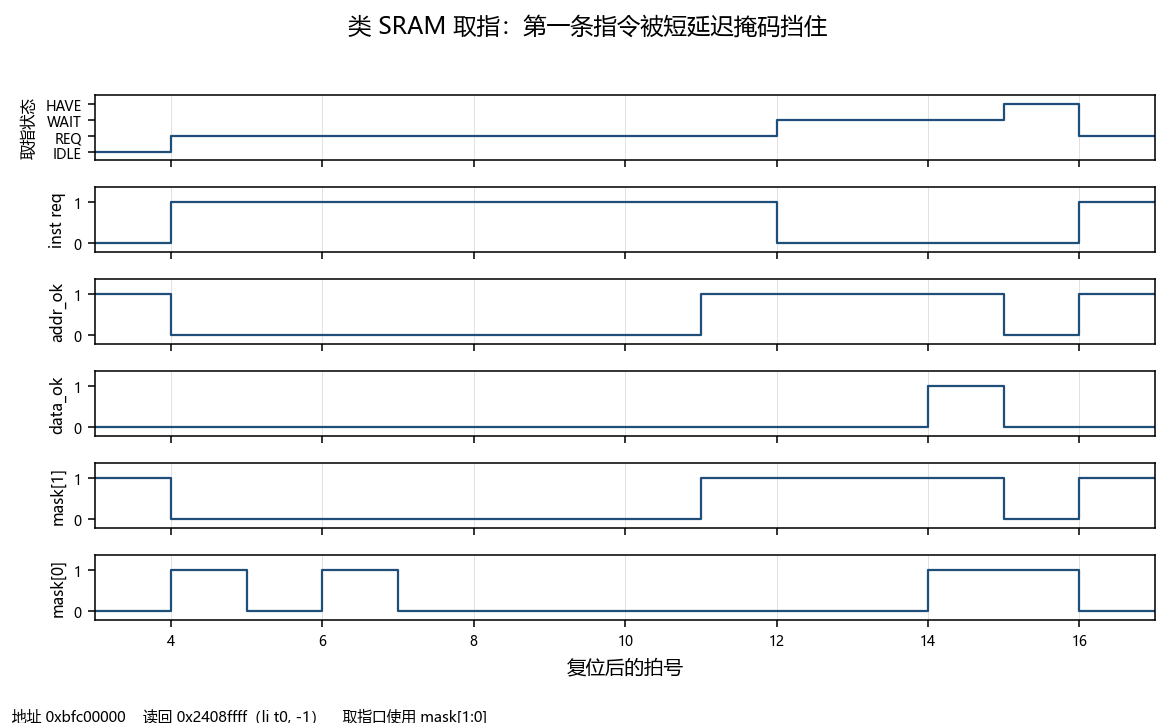
\includegraphics[width=0.92\textwidth]{fig/sram_fetch.png}
\caption{短设置下首条取指：\texttt{req} 自第 4 个时钟周期保持至第 11 个时钟周期获得 \texttt{addr\_ok}，\texttt{data\_ok} 于第 14 个时钟周期。}
\end{figure}

\subsection{延迟槽}
第 23 个时钟周期 \texttt{S\_HAVE} 的 PC 是 \texttt{0xbfc00008}，指令 \texttt{0x100001ab}，即 \texttt{b locate}。
第 24 个时钟周期这条分支进入译码级，\texttt{ds\_is\_bj} 为 1，\texttt{wait\_bd} 为 1，\texttt{br\_taken} 为 0。
取指口改为请求延迟槽 \texttt{0xbfc0000c}，该时钟周期 \texttt{addr\_ok} 为 1。
第 25 个时钟周期 \texttt{data\_ok} 返回，\texttt{wait\_bd} 仍为 1。
第 26 个时钟周期 \texttt{nop} 进入 \texttt{S\_HAVE}，\texttt{fs\_pc} 等于译码级 PC 加 4，\texttt{wait\_bd} 变为 0，\texttt{br\_taken} 为 1。
第 27 个时钟周期下一次请求地址是 \texttt{0xbfc006b8}。
bit 1 在第 27 个到第 32 个时钟周期为 0，第 33 个时钟周期 \texttt{addr\_ok} 才为 1。
第 35 个时钟周期锁存 \texttt{0x3c04bfb0}，即 \texttt{locate} 处的 \texttt{lui a0, 0xbfb0}。

\begin{figure}[H]
\centering
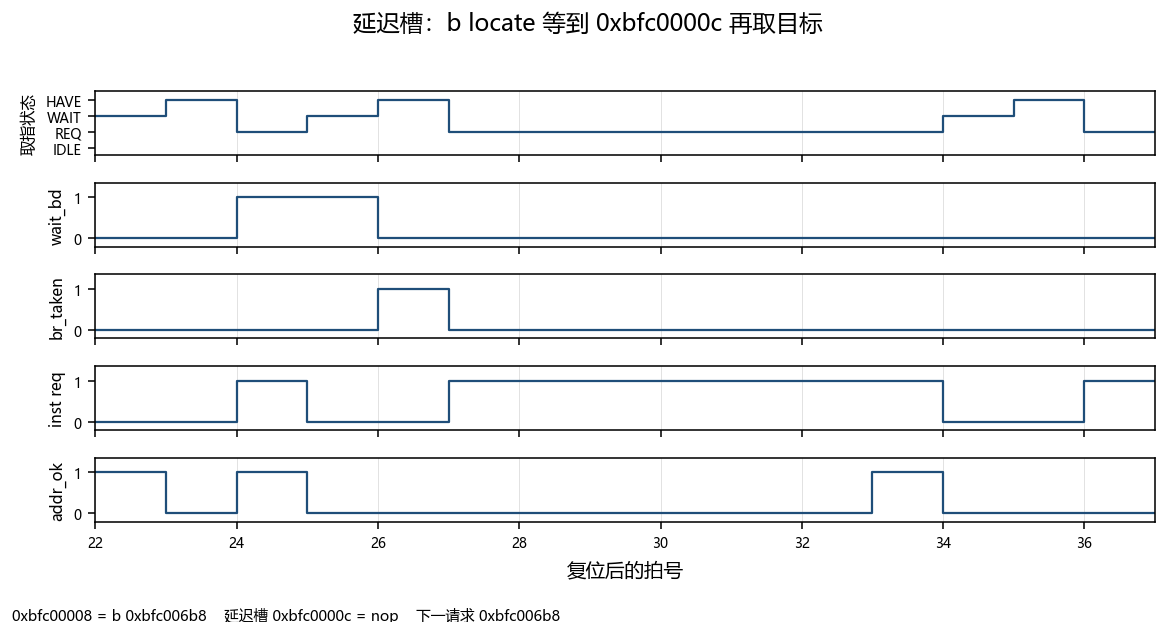
\includegraphics[width=0.92\textwidth]{fig/sram_delay.png}
\caption{延迟槽：第 26 个时钟周期 \texttt{br\_taken} 成立，下一请求地址已切换为 \texttt{0xbfc006b8}。}
\end{figure}

\subsection{写 confreg}
第一条 \texttt{sw} 是 \texttt{sw t1, 0(a0)}。
第 142 个时钟周期它已经在执行级：\texttt{wr} 为 1，地址 \texttt{0xbfaff008}，数据 \texttt{0x2}，写选通 \texttt{0xf}。
\texttt{bridge\_1x2} 把 \texttt{0xbfaff008} 送到 confreg，而 confreg 的 \texttt{addr\_ok} 固定为 1，
所以数据口的 \texttt{addr\_ok} 在请求发出之前已经为 1。
第 143 个时钟周期进入 \texttt{D\_REQ}，\texttt{req} 为 1，并在该时钟周期被接受。
第 144 个时钟周期处于 \texttt{D\_WAIT}，\texttt{data\_ok} 为 1。
第 145 个时钟周期进入 \texttt{D\_DONE}。
第 148 个到第 149 个时钟周期是下一条 \texttt{sw t2, 0(a1)}，地址 \texttt{0xbfaff004}，数据 \texttt{0x1}。

\begin{figure}[H]
\centering
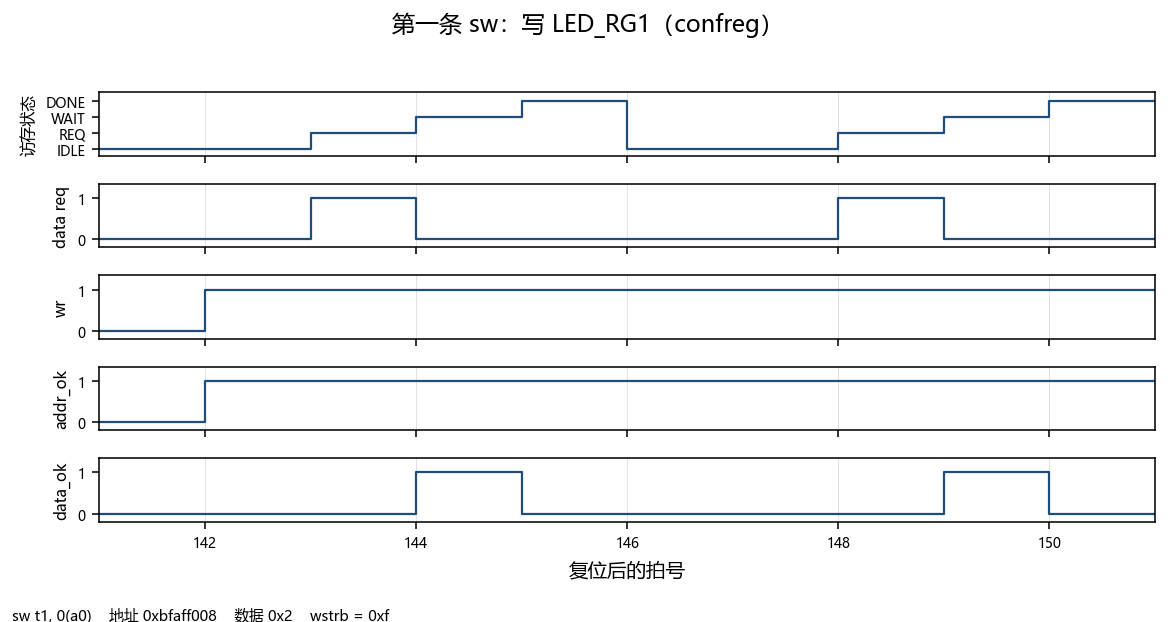
\includegraphics[width=0.92\textwidth]{fig/sram_store.png}
\caption{写 confreg（LED\_RG1）：\texttt{addr\_ok} 与请求在同一时钟周期，\texttt{data\_ok} 在下一时钟周期。}
\end{figure}

\subsection{AXI 读}
固定设置下掩码保持 \texttt{5'b11111}。
第 4 个时钟周期取指进入 \texttt{S\_REQ}，\texttt{req} 与 \texttt{addr\_ok} 同为 1。
转换器仍在 \texttt{A\_IDLE}，\texttt{addr\_ok} 由 \texttt{req} 组合得到。
第 5 个时钟周期 CPU 进入 \texttt{S\_WAIT}，转换器进入 \texttt{A\_AR}，\texttt{arvalid} 为 1，\texttt{arready} 为 0。
第 7 个时钟周期 \texttt{arready} 为 1，主端口 \texttt{arvalid} 为 1，\texttt{arid} 为 0。
第 8 个时钟周期进入 \texttt{A\_R}，\texttt{rready} 为 1。
第 12 个时钟周期 \texttt{rlast} 为 1，读数据线上已经是 \texttt{0x2408ffff}，\texttt{rvalid} 仍为 0。
第 13 个时钟周期 \texttt{rvalid}、\texttt{rready}、\texttt{rlast} 同时为 1，\texttt{data\_ok} 为 1。
第 14 个时钟周期转换器回到 \texttt{A\_IDLE}，取指进入 \texttt{S\_HAVE}。

\begin{figure}[H]
\centering
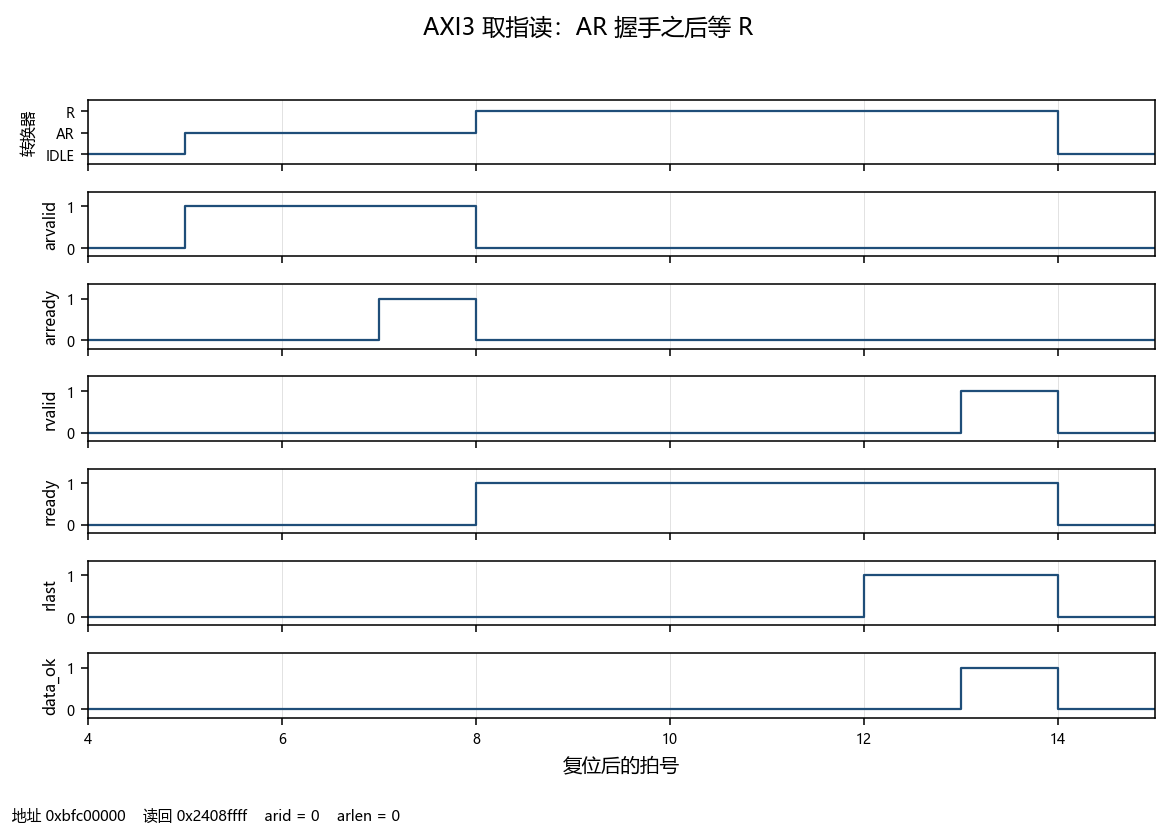
\includegraphics[width=0.92\textwidth]{fig/axi_read.png}
\caption{首条指令的 AXI 读：AR 于第 7 个时钟周期、R 于第 13 个时钟周期完成握手。}
\end{figure}

\subsection{AXI 写}
第 189 个时钟周期数据转换器进入 \texttt{A\_WRITE}。
\texttt{awvalid} 与 \texttt{wvalid} 同时为 1，地址 \texttt{0xbfaff008}，数据 \texttt{0x2}，\texttt{wstrb} 为 \texttt{0xf}。
第 191 个时钟周期 \texttt{awready} 为 1，主端口 \texttt{awid} 为 8，\texttt{wready} 仍为 0。
\texttt{aw\_done} 记住地址通道已经握手，第 192 个时钟周期 \texttt{awvalid} 拉低，\texttt{wvalid} 继续保持。
第 193 个时钟周期 \texttt{wready} 为 1。
第 194 个时钟周期进入 \texttt{A\_WRESP}，\texttt{bready} 为 1。
第 198 个时钟周期 \texttt{bvalid} 为 1。
第 199 个时钟周期回到 \texttt{A\_IDLE}，执行级进入 \texttt{D\_DONE}。

\begin{figure}[H]
\centering
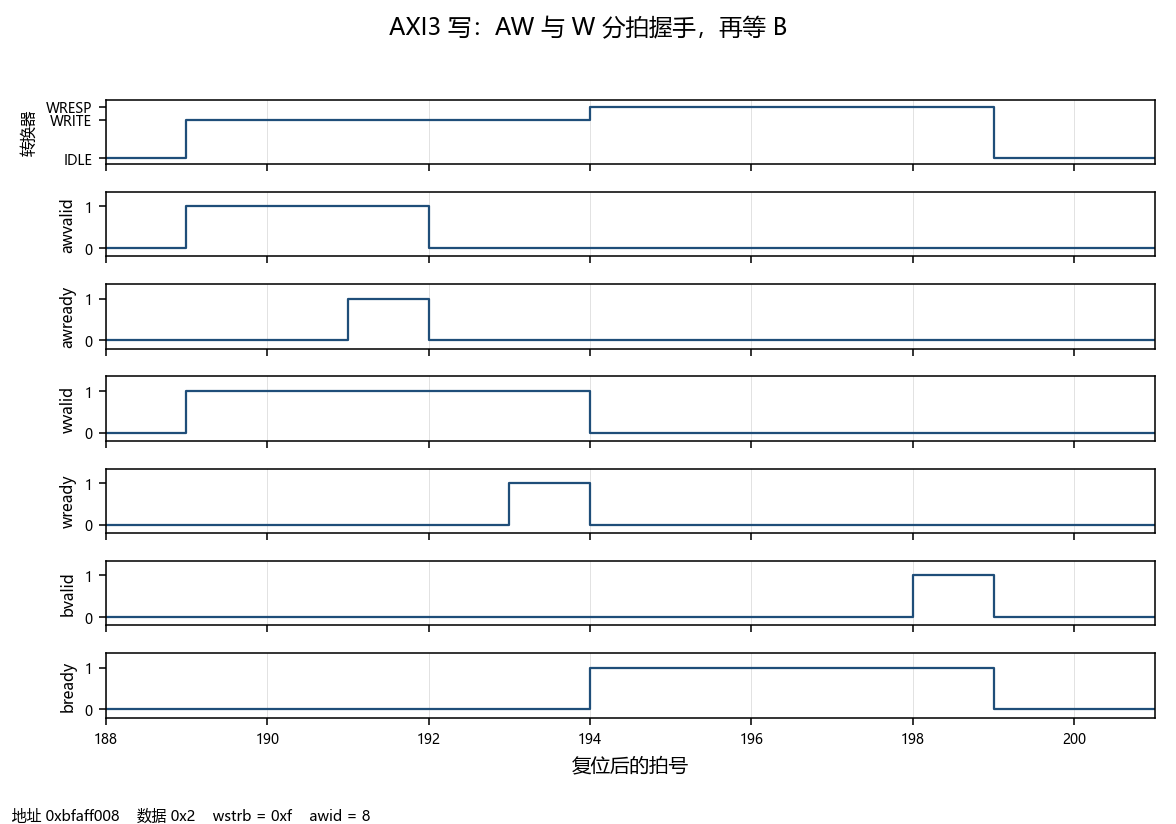
\includegraphics[width=0.92\textwidth]{fig/axi_write.png}
\caption{首条 \texttt{sw} 的 AXI 写：AW/W/B 分别在第 191、193、198 个时钟周期握手。}
\end{figure}

第 216 个时钟周期主端口上 \texttt{arvalid} 与 \texttt{awvalid} 同时为 1。
\texttt{arid} 为 0，对应取指地址 \texttt{0xbfc00704}；\texttt{awid} 为 8，对应写地址 \texttt{0xbfaff000}。
取指转换器停在 \texttt{A\_AR}，该时钟周期自己的 \texttt{arready} 到来后进入 \texttt{A\_R}。
数据转换器的 AW 已经结束，W 通道仍为 1，随后进入 \texttt{A\_WRESP}。
第 226 个时钟周期再次重叠：取指读 \texttt{0xbfc00708}，同时写 \texttt{0xbfaff010}。
同一主端口上读、写通道可并行占用；R/B 凭基址 ID 回到对应的转换器端口。

\begin{figure}[H]
\centering
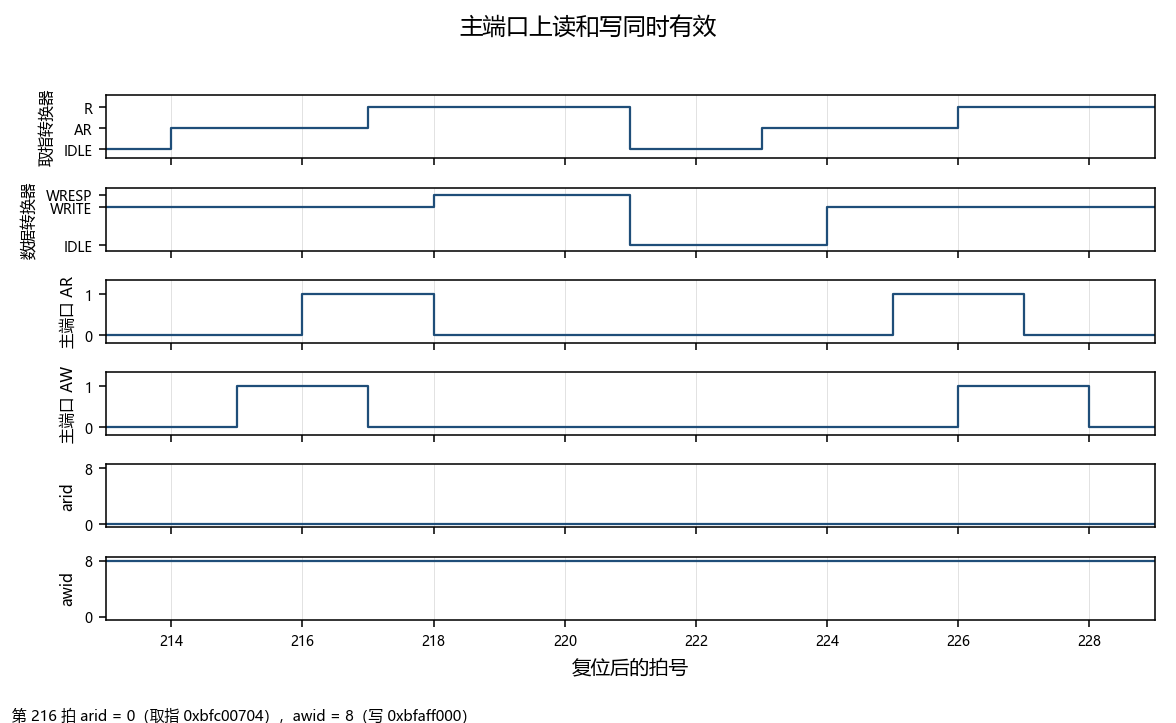
\includegraphics[width=0.92\textwidth]{fig/axi_both.png}
\caption{读、写重叠：第 216 个与第 226 个时钟周期主端口 AR、AW 同时有效（\texttt{arid}=0，\texttt{awid}=8）。}
\end{figure}

\section {实验收获}
本实验复用实验 3 已经调试完成的五级流水线、CP0、异常与中断内核逻辑，核心工作不改动核内通路，而是对处理器对外总线接口进行改造，依托同一套 \texttt {func\_lab9} 写回 trace 作为功能参照，在总线架构迭代的过程中验证内核行为的稳定性。

任务一的工作是把顶层接口重构为类 SRAM 两段握手协议，单次访问拆分为 \texttt {addr\_ok} 和 \texttt {data\_ok} 两个阶段，同时约束取指、访存端口各自最多保留一笔在途传输。这一阶段的调试重心，是建立两段握手之间的绑定关系，保证地址握手和数据握手能够匹配到同一次请求。我采用的实现方式是：\texttt {addr\_ok} 拉高的下一拍就撤销 \texttt {req}，让 \texttt {sram\_wrap} 只接收一次地址握手；而 \texttt {data\_ok} 至少延后一拍，绑定最近一次已经被接收的请求。流水线清空场景是这里最容易出 bug 的地方：需要区分两类请求，还没有被接收的请求允许修改地址，已经完成地址握手的请求则必须等待 \texttt {data\_ok}，只是收到数据后直接丢弃。与之配套的分支约束也需要同步梳理，\texttt {br\_taken} 不能过早更新分支目标，要等到取指级 PC 和当前指令 PC+4 对齐之后再跳转，保证延迟槽指令会先于分支目标指令出现在取指口，这部分时序约束需要和握手逻辑一起对齐，很容易因为一拍偏差引发隐性错误。

任务二在核外新增 \texttt {sram2axi} 转接桥，把这套两段式握手封装成标准 AXI3 事务，再将独立的取指、访存两路请求合并成单一 AXI 主端口。转接桥本质上是协议转换层，要把简单的握手语义翻译成 AXI 的五条通道握手机制。这里需要遵守 AXI 的基本规则：\texttt {arvalid}、\texttt {awvalid}、\texttt {wvalid} 置高之后必须保持，直到从端给出对应的 ready。同时要处理流水线清空和 AXI 事务的冲突：一旦通道上事务已经发起，就不能中途打断，必须让事务完整走完，只在收到 R 读响应或者 B 写响应之后丢弃结果，而不是直接掐断事务。取指和访存有可能同时发出请求，我用基 ID 0 和 8 来标记事务来源，保证响应能够原路送回，实现读写通道并行工作。协议转换的一层封装，天然会引入固定的一拍延时，这也让我体会到不同总线抽象之间的代价：简洁的握手接口对内核友好，但向外映射到 AXI 时，时序开销会藏在桥接逻辑里。

任务三设计了对照路径，独立实现原生 AXI 通路作为对比基准：内核流水线直接驱动 AXI 五条通道，不再经过类 SRAM 握手与转接桥，对外维持相同的 AXI3 主端口。我通过修改 \texttt {RANDOM\_SEED} 低 16 位，在固定、短随机、长随机三种延迟配置下，依次跑通类 SRAM 直连、转接桥、原生 AXI 三组通路。随机延迟的作用是扰动握手发生的时钟位置，用来检验设计是不是只在特定时序下碰巧正确，而不是真正满足协议约束。调试过程中，我借助复位后前 4500 个时钟周期的波形，把转接桥带来的固定封装延时、从设备随机等待延时拆开分析，对比转接桥和原生 AXI 通路里 \texttt {arready} 到 \texttt {rlast} 的链路延时，理解协议转换带来的开销到底落在哪个环节。

整个实验让我对分层接口思想有了更直观的感受：内核本身的流水线、异常、中断逻辑可以稳定不变，上层总线只是一层交换外壳。不管是两段式 SRAM 握手，还是 AXI 复杂通道，只要接口契约被严格遵守，内核的功能行为就可以保持一致。Count、Compare 寄存器依旧由 \texttt {mtc0} 配置，定时器与软件中断依然落在原地循环 \texttt {b 1b} 和它的延迟槽 \texttt {nop} 上，这也印证了总线属于外设交互层，不会侵入异常中断的内核机制。

调试里最深刻的体会是，很多错误不是逻辑写错，而是对 “请求生命周期” 的边界处理不周：什么时候可以取消请求、什么时候事务必须跑完、清空流水线时哪些信号要保留、哪些结果要丢弃，这些边界场景在理想时序下很难暴露，只有引入随机延迟之后，才会把时序上的漏洞翻出来。同时对比转接桥和原生 AXI 两条实现路线，也让我看清两种工程取舍：桥接方案对内屏蔽复杂 AXI 细节，便于内核迭代；原生 AXI 通路减少协议转换开销，但会把 AXI 通道的时序负担直接压到流水线各级，两者各有适用场景。

\section{附：源码目录}
类 SRAM 的 CPU 在 \texttt{CPU\_CDE\_SRAM} 的 \texttt{myCPU} 目录。
AXI 工程引用这些核心文件，顶层和转换器在 \texttt{CPU\_CDE\_AXI}。
\begin{itemize}
\item \verb|lab4/CPU_CDE_SRAM/mycpu_sram_verify/rtl/myCPU/IF_stage.v|
\item \verb|lab4/CPU_CDE_SRAM/mycpu_sram_verify/rtl/myCPU/ID_stage.v|
\item \verb|lab4/CPU_CDE_SRAM/mycpu_sram_verify/rtl/myCPU/EXE_stage.v|
\item \verb|lab4/CPU_CDE_SRAM/mycpu_sram_verify/rtl/myCPU/mycpu_core.v|
\item \verb|lab4/CPU_CDE_SRAM/mycpu_sram_verify/rtl/myCPU/mycpu_top.v|
\item \verb|lab4/CPU_CDE_AXI/mycpu_axi_verify/rtl/myCPU/mycpu_top.v|
\item \verb|lab4/CPU_CDE_AXI/mycpu_axi_verify/rtl/myCPU/sram_axi_bridge.v|
\item \verb|lab4/CPU_CDE_AXI/mycpu_axi_verify/rtl/myCPU/if_stage_axi.v|
\item \verb|lab4/CPU_CDE_AXI/mycpu_axi_verify/rtl/myCPU/exe_stage_axi.v|
\item \verb|lab4/CPU_CDE_AXI/mycpu_axi_verify/rtl/myCPU/mycpu_core_axi.v|
\item \texttt{axi\_crossbar\_2x1} 在
      \texttt{CPU\_CDE\_AXI/mycpu\_axi\_verify/rtl/xilinx\_ip} 下
\item \verb|lab4/CPU_CDE_AXI/mycpu_axi_verify/rtl/CONFREG/confreg.v|
\item \verb|lab4/CPU_CDE_SRAM/cpu132_gettrace/golden_trace.txt|
\item \verb|lab4/sim/sram_wave.csv|
\item \verb|lab4/sim/axi_wave.csv|
\item \verb|lab4/sim/native_wave.csv|
\item \verb|lab4/sim/plot_wave.py|
\item \verb|lab4/report/fig/|
\item \verb|lab4/report/report.tex|
\end{itemize}
\texttt{sram\_axi\_bridge.v} 里的模块名是 \texttt{sram2axi}，取指和数据各例化一次。

\end{document}
